% Created 2023-09-17 dom 20:52
% Intended LaTeX compiler: pdflatex
\documentclass[11pt]{article}
\usepackage[utf8]{inputenc}
\usepackage[T1]{fontenc}
\usepackage{graphicx}
\usepackage{grffile}
\usepackage{longtable}
\usepackage{wrapfig}
\usepackage{rotating}
\usepackage[normalem]{ulem}
\usepackage{amsmath}
\usepackage{textcomp}
\usepackage{amssymb}
\usepackage{capt-of}
\usepackage{hyperref}
\usepackage{../../modern}
\bibliography{../../sample.bib}
\raggedbottom
\setcounter{secnumdepth}{2}
\author{Héctor Miguel Macías Baltazar  (1272124) \\
Luis Eduardo Galindo Amaya  (1274895)}
\date{16 de Septiembre 2023}
\title{Práctica No. 2 Laboratorio}
\hypersetup{
 pdfauthor={Héctor Miguel Macías Baltazar  (1272124) \\
Luis Eduardo Galindo Amaya  (1274895)},
 pdftitle={Práctica No. 2 Laboratorio},
 pdfkeywords={},
 pdfsubject={},
 pdfcreator={Emacs 27.1 (Org mode 9.3)}, 
 pdflang={Spanish}}
\begin{document}

\modentitlepage{../../images/escudo-uabc-2022-color-cont.png}
\thispagestyle{empty}\tableofcontents\pagebreak
\datasection{En equipo} 

\section{Detalles de la práctica}
\label{sec:org12a807d}
\subsection{Competencia}
\label{sec:org2bcc8c5}
Implementar un sistema inteligente, mediante agentes de software, para la abstracción de sus unidades principales, con una actitud creativa y crítica.

\subsection{Descripción}
\label{sec:org0fcbbd4}
Analiza, diseña e implementa una solución de un problema propuesto, mediante un enfoque orientado a agentes inteligentes. Elaborar y entregar un reporte donde se describa el análisis, diseño e implementación de la solución propuesta.

\subsection{Procedimiento}
\label{sec:orgd7a65df}
En equipos de máximo dos personas:
\begin{enumerate}
\item Elegir una plataforma de desarrollo de agentes autónomos inteligentes.
\item Implementar la simulación propuesta, y aprobada, en la Práctica de Taller No. 2.
\item Elaborar un reporte técnico de lo hecho.
\end{enumerate}

\section{Introducción}
\label{sec:org8bbf995}
La Inteligencia Artificial se ha convertido en una herramienta crucial para mejorar la eficiencia y la productividad en toda la industria. La capacidad de modelar y simular procesos complejos a través de agentes ha llevado a la investigación en la optimización de sistemas de producción y logística. En este contexto, nuestro proyecto se enfoca en la creación de una simulación de una línea de ensamblaje básica con el propósito de explorar cómo los agentes pueden mejorar la gestión de procesos industriales.

\subsection{Problema}
\label{sec:org9d389d2}
Uno de los sectores más importantes de la industria en Tijuana es la fabricación y ensamblaje de productos que serán exportados a los Estados Unidos. Conocer la cantidad de gente que es necesaria para el proceso de ensamblaje es muy útil para maximizar la eficiencia, reducir la cantidad de operadores por línea a los estrictamente necesarios y maximizar la cantidad de ingresos.

\subsection{Propuesta}
\label{sec:org9d1d96c}
Para ayudar a optimizar los procesos de ensamblaje nosotros proponemos crear un simulador de una linea de ensamble, en la cual se puedan manipular los parámetros de cada estación y de cada operador para ver como se desempeñan los
operadores en la nueva situación.

\begin{figure}[htbp]
\centering
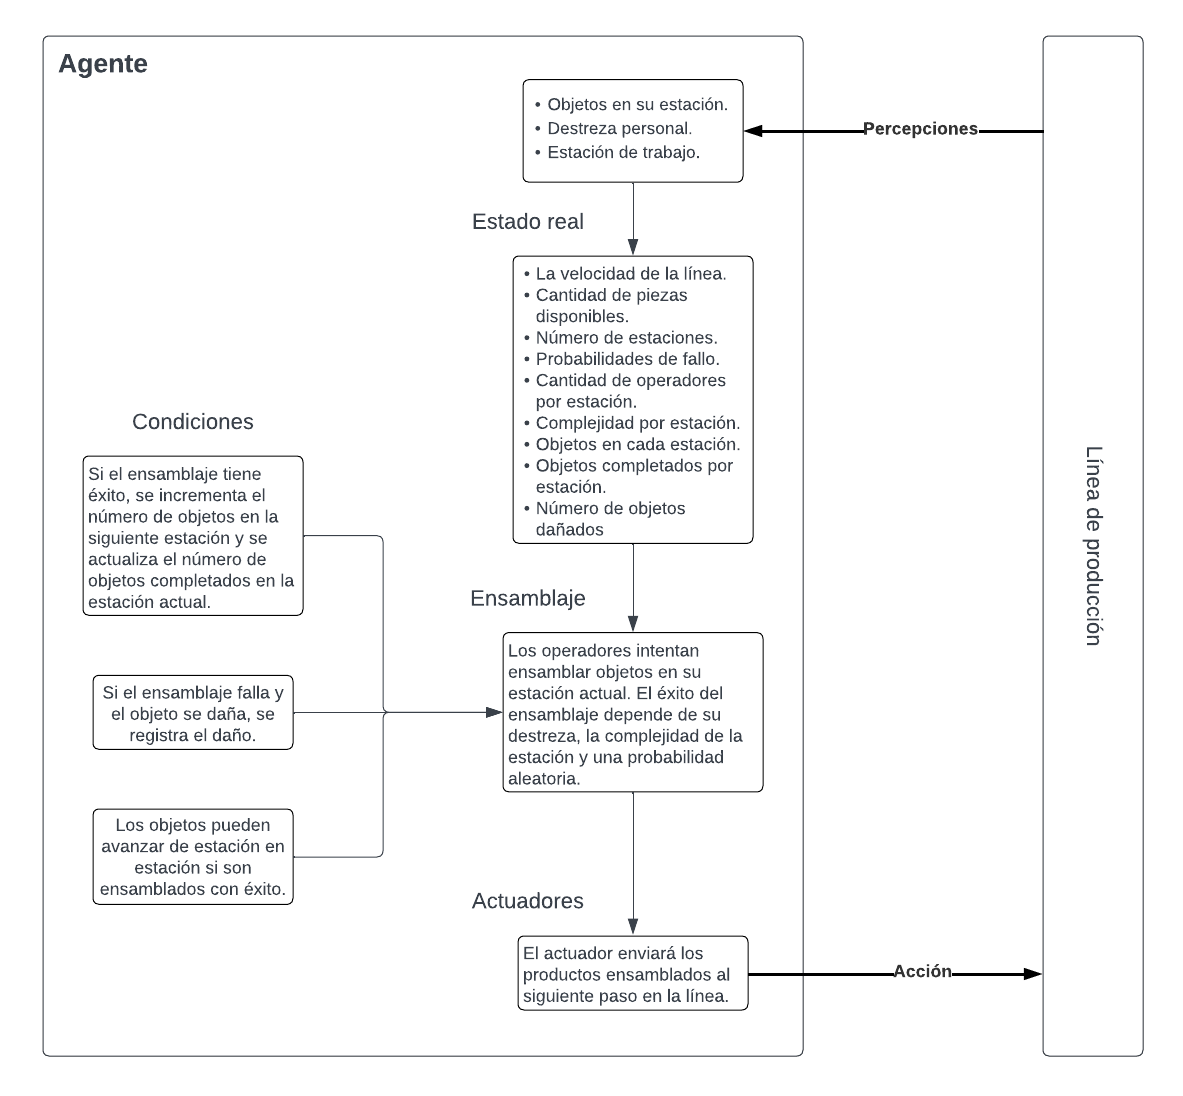
\includegraphics[width=.9\linewidth]{img/diagrama.png}
\caption{Propuesta de la arquitectura}
\end{figure}

\section{Arquitectura}
\label{sec:orgff29a8a}
\subsection{Pieza}
\label{sec:org10bb4b3}
Una pieza es uno de los procesos que intentara hacer el operador, se puede interpretar la pieza como uno de los elementos en la línea de ensamble, una pieza se dice que está terminada cuando pasa por la última estación sin romperse en el proceso. 

\subsection{Operador}
\label{sec:org259feee}
El operador solo tiene una variable, la \textbf{Destreza,} la cual se asigna al azar, al iniciar la simulación esta puede ir del 0 al 100, donde 0 es el mínimo de destreza y 100 el máximo. 

\subsection{Estación}
\label{sec:orgfed658e}
Una estación representa un paso dentro de la línea de ensamble, cada paso tiene:

\begin{itemize}
\item Número de agentes en cada estación
\item Destreza mínima requerida
\item Probabilidad que dañar la pieza
\end{itemize}

\section{Desarrollo}
\label{sec:org0e7145d}
\subsection{Procesamiento de las piezas}
\label{sec:org8e5b20c}
Al procesar la pieza hay 3 posibles escenarios que se pueden dar:
\begin{description}
\item[{Se completó con éxito}] La pieza pasa por la estación sin problemas
\item[{Falló y la pieza se dañó}] al pasar por la estación se daño y se tiene que descartar por completo
\item[{Falló, pero la pieza no se daño}] no se completo con éxito, pero se puede volver a intentar solo que habrá retraso en la próxima estación
\end{description}

\begin{verbatim}
ifelse
(random 100 * (dexterity / 100)) >= station-complexity [
  ; se completo con exito...
]

random 100 < array:item falure-rates station [
  ; falló y la pieza se daño...
]

[
  ; falló pero la pieza no se daño...
]
\end{verbatim}

\subsection{Ajustar la dificultad de cada estación}
\label{sec:org8e847a4}
El simulador esta limitado únicamente a cuatro estaciones, cada estación tiene dos variables, la complejidad y la probabilidad de fallo

\begin{figure}[htbp]
\centering
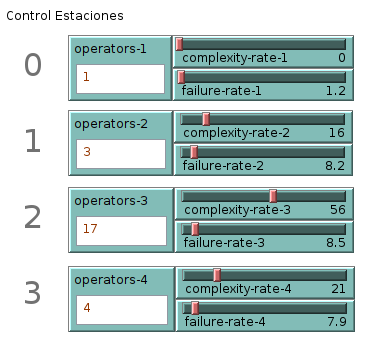
\includegraphics[width=6 cm]{img/stations.png}
\caption{Ajuste de parámetros de la estación}
\end{figure}


\subsection{Creación de los agentes (Operadores)}
\label{sec:org9681f32}
Para desarrollar nuestro sistema de agentes decidimos usar Netlogo, ya que nos brinda una mayor facilidad para crear y manipular agentes de manera rápida. Los operadores se representan como 'tortugas' de netlogo:

\begin{verbatim}
breed [operator operators]
operator-own [
  station                  ;Estacion de trabajo
  dexterity                ;Destreza
  completed                ;Objetos completados
]
\end{verbatim}

Utilizando el método \texttt{create-operador} se crea un nuevo operador y se le asigna una destreza aleatoria mediante el método \texttt{calc-dexterity}

\begin{verbatim}
create-operator 1 [
  setxy xcoord ycoord
  set color white
  set shape "square"
  set size 1

  set dexterity (calc-dexterity)
  set station n-station
]

to-report calc-dexterity
  ; Calcula la destreza para cada agente

  if fix-dexterity [
    report fixed-dexterity
  ]

  report (base-dexterity 
    + (range-random (- variance-dexterity) variance-dexterity))
end
\end{verbatim}

\subsection{Análisis de sensibilidad económica}
\label{sec:org8616b48}
En la parte inferior de la interfaz se encuentra la sección de sensibilidad económica, la cual muestra cuanto valor se puede extraer del proceso:

\begin{figure}[htbp]
\centering
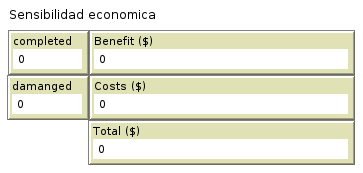
\includegraphics[width=6cm]{img/sensibilidad.png}
\caption{Análisis de sensibilidad}
\end{figure}

El análisis es bastante básico, calcula la diferencia entre el valor que se ganó con las piezas contra el valor de las piezas que se descartaron, para esto se usan dos parámetros:

\begin{figure}[htbp]
\centering
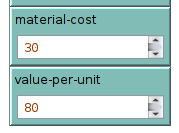
\includegraphics[width=4cm]{img/vars.png}
\caption{Variables del análisis}
\end{figure}

\begin{description}
\item[{material-cost}] costo en material para la pieza
\item[{value-per-unit}] valor de venta de la pieza
\end{description}

El valor neto de la pieza se calcula mediante la siguiente fórmula:

\[
\textrm{valorNeto} = \textrm{materialCost} - \texttextrm{valuePerUnit}
\]
\subsection{Gráfica de producción throttling}
\label{sec:org66ebd33}
En esta gráfica se representa en que estación se está quedando atoradas las piezas, por ejemplo si en la gráfica hay una línea muy alta esto podría significar que faltan operadores es en esa estación.

\begin{figure}[htbp]
\centering
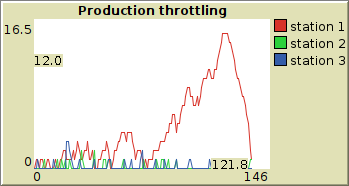
\includegraphics[width=6cm]{img/pt.png}
\caption{Las piezas se atoran mucho en la estación 1}
\end{figure}

\section{Capturas del simulador}
\label{sec:orgee2b126}

\begin{figure}[htbp]
\centering
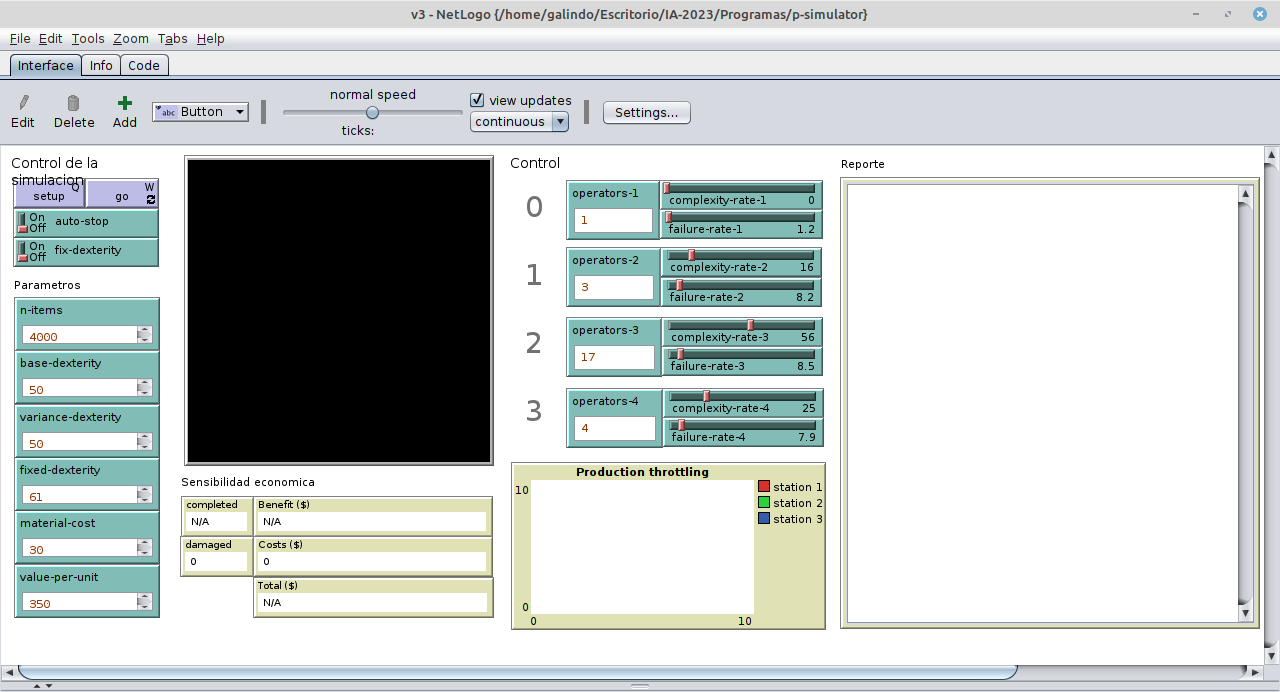
\includegraphics[width=9.5cm]{img/sim1.png}
\caption{Primera pantalla del simulador}
\end{figure}

\begin{figure}[htbp]
\centering
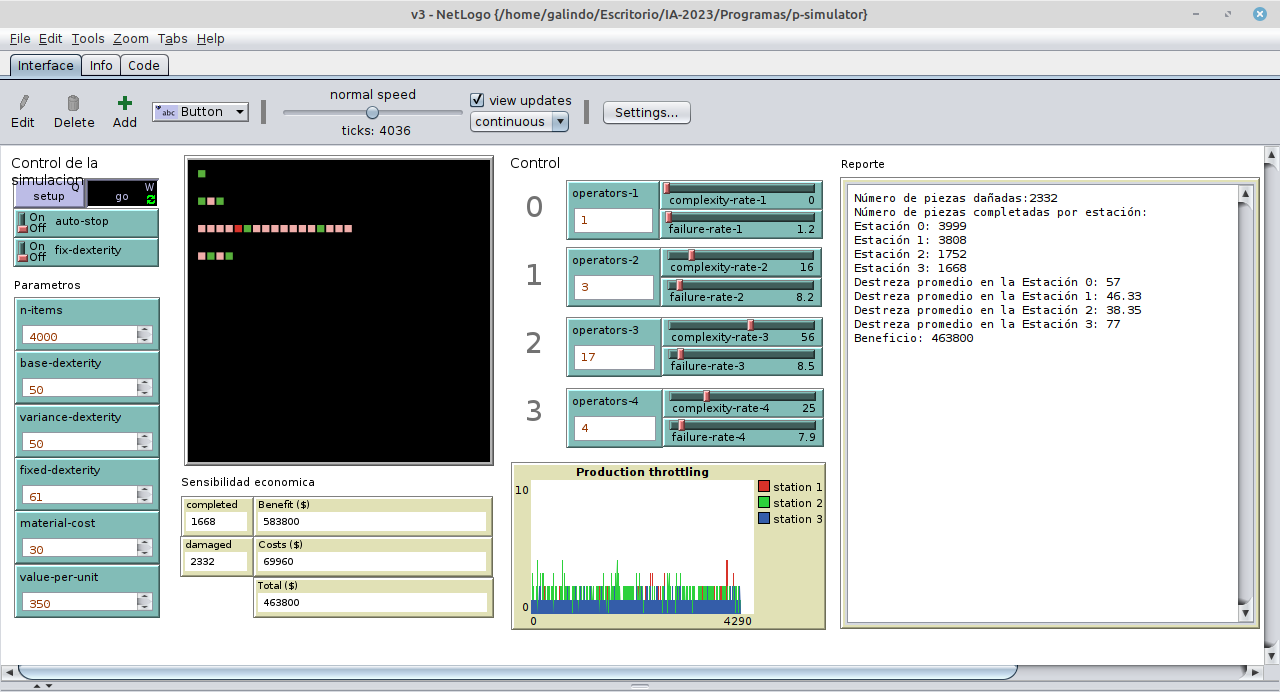
\includegraphics[width=9.5cm]{img/sim2.png}
\caption{Simulador después de la simulación}
\end{figure}

\section{Código del simulador}
\label{sec:org624f9ef}
Una copia del código se puede encontrar en:
\begin{itemize}
\item \url{https://github.com/IA-Galindo-Macias/p-simulator/blob/main/v3.nlogo}
\end{itemize}

\begin{verbatim}
extensions [
  array
]

globals [
  failure-rates            ;lista de probabilidades de fallo
  operators-station        ;operadores por estacion
  stations-delay-rate      ;probabilidad de retrasos por estacion
  objects-stage            ;objetos por estacion
  stations-complexity-rate ;complejidad de la estacion
  n-stations               ;numero de estaciones
  damaged                 ;numero de equipos dañados
  printed                  ;valor impreso
  completed-items-set      ; conjunto de arreglos para objetos completados por estación
]

breed [operator operators]
operator-own [
  station                  ;indice de la estacion de trabajo
  dexterity                ;destreza
  completed                ;objetos completados
]

to setup
  clear-all
  set n-stations 4
  set damaged 0
  set objects-stage array:from-list (list n-items 0 0 0 0)

  ; Inicializa completed-items-set con valores iniciales de 0
  set completed-items-set array:from-list (list 0 0 0 0)

  set failure-rates array:from-list
  ( list
    failure-rate-1
    failure-rate-2
    failure-rate-3
    failure-rate-4
  )

  set operators-station array:from-list
  ( list
    operators-1
    operators-2
    operators-3
    operators-4
  )

  set stations-complexity-rate array:from-list
  ( list
    complexity-rate-1
    complexity-rate-2
    complexity-rate-3
    complexity-rate-4
  )

  create-assembly-line

  ; reiniciar ticks
  reset-ticks
end


to create-assembly-line
  ; crear los operadores
  let xcoord -15
  let ycoord 15
  let n-station 0

  repeat n-stations
  [
    let n-operators (array:item operators-station n-station)

    repeat n-operators
    [
      create-operator 1
      [
        setxy xcoord ycoord
        set color white
        set shape "square"
        set size 1
        set dexterity (calc-dexterity)
        set station n-station
        set completed 0 ; Agregar esta linea para inicializar completed
      ]

      set xcoord (xcoord + 1)
    ]

    set xcoord -15
    set ycoord (ycoord - 3)
    set n-station (n-station + 1)
  ]
end


to-report range-random [minnumber maxnumber]
  ; Genera un numero aleatorio entre [minnumber] y [maxnumber]

  report minnumber + (random (maxnumber - minnumber))
end



to-report calc-dexterity
  ; Calcula la destreza para cada agente

  if fix-dexterity
  [
    ; si la destreza esta fijada
    report fixed-dexterity
  ]

  report base-dexterity + (range-random (- variance-dexterity) variance-dexterity)
end


to go
  ask operator
  [
    let obj-current-station (array:item objects-stage station)


    ; verificar que hay objetos en la linea
    if obj-current-station > 0
    [
      ; verificar si se pudo ensamblar la pieza
      let station-complexity array:item stations-complexity-rate station


      (ifelse
        ; se completo con exito
        (random 100 * (dexterity / 100)) > station-complexity
        [
          set color green
          ; incrementar los valores en la siguiente estacion
          let obj-next-station    array:item objects-stage (station + 1)
          array:set objects-stage station (obj-current-station - 1)
          array:set objects-stage (station + 1) (obj-next-station + 1)

          ; Actualizar el numero de objetos completados en esta estacion
          let completed-items array:item completed-items-set station
          array:set completed-items-set station (completed-items + 1)
        ]


        ; fallo y la pieza se daño
        random 100 < array:item failure-rates station
        [
          set color red
          array:set objects-stage station (obj-current-station - 1)
          set damaged (damaged + 1)
        ]


        ; fallo pero la pieza no se daño
        [
          set color 18
        ])
    ]
  ]

  ; revisar si el numero de objetos es igual al procesado
  ifelse procesed-items = n-items
  [

    if printed
    [
      print total-benefits
      print-report  ; Llama al procedimiento para imprimir el informe

      set printed false
    ]

    if auto-stop
    [
      stop
    ]


  ]
  [
    set printed true
    tick
  ]


end

to-report procesed-items
  report (array:item objects-stage n-stations) + damaged
end

to-report total-benefits
  report (value-per-unit - material-cost) * (array:item objects-stage 4) - damaged * material-cost
end

to print-report
  ; Imprimir el numero de piezas dañadas
  output-print (word "Número de piezas dañadas:" damaged) ; sí imprime tildes lol
  ;output-print damaged

  ; Imprimir el numero de piezas completadas por estacion
  output-print "Número de piezas completadas por estación:"
  foreach [0 1 2 3] [ station-index ->
      ;let completed-items (array:item objects-stage station-index) ; No sirve, imprime 0
      output-print (word "Estación " station-index ": " array:item completed-items-set station-index)
  ]

  ; Calcular e imprimir la destreza promedio por estacion
  let total-dexterity 0
  foreach [0 1 2 3] [station-index ->
    let total-dexterity-per-station sum [dexterity] of operator with [station = station-index]
    let average-dexterity-per-station total-dexterity-per-station / array:item operators-station station-index
    output-print (word "Destreza promedio en la Estación " station-index ": " precision average-dexterity-per-station 2)
    set total-dexterity total-dexterity + total-dexterity-per-station
  ]

  ; Imprimir el balance de la relacion costo-beneficio
  output-print (word "Beneficio: " total-benefits)
end





\end{verbatim}

\pagebreak

\section{Conclusión}
\label{sec:orgf2c9b3b}
Hemos aprendido cómo modelar operadores como agentes individuales en una simulación. Representar la destreza como un atributo de un operador nos ha permitido observar cómo el comportamiento individual de los operadores puede dar lugar a un comportamiento emergente a nivel del sistema. Las interacciones entre los operadores, la tasa de fallos y la complejidad de las estaciones contribuyen al rendimiento general de la línea de producción. \\

La introducción de aleatoriedad en la simulación, como las probabilidades de fallo y las destrezas variables, refleja la naturaleza casual de los procesos reales y nos permite explorar escenarios realistas. En otras palabras, esta simulación de agentes ha destacado la utilidad de del modelado basado en agentes para comprender y analizar procesos industriales complejos, no sin antes mencionar la funcionalidad general de los agentes.
\end{document}
